\renewcommand{\mapa}{Poglavja/Slike/kompleksnost}

\begin{figure}
    \begin{subfigure}{0.5\linewidth}
        
\includegraphics[width=\linewidth]{\mapa/preprosta grayscale 300/knjiga.png}
        \caption{Slika s preprostim motivom}
    \end{subfigure}
    \hfill
    \begin{subfigure}{0.5\linewidth}
        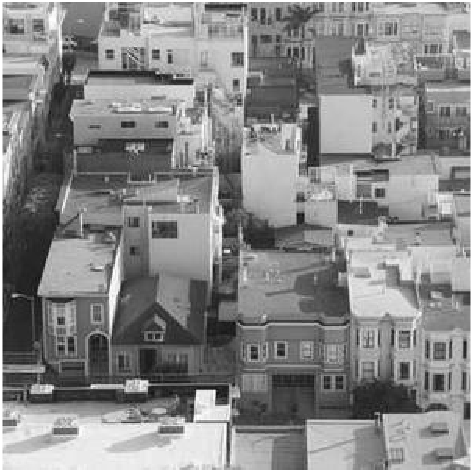
\includegraphics[width=\linewidth]{\mapa/kompleksna grayscale 300/mesto.png}
        \caption{Slika s kompleksnim motivom}
    \end{subfigure}
    \caption{Vir slik: Unsplash}
\end{figure}

\begin{figure}
    \begin{subfigure}{0.325\linewidth}
        \includegraphics[width=\linewidth]{\mapa/preprosta grayscale 300/rez35SVT.png}
    \end{subfigure}
    \hfill
    \begin{subfigure}{0.325\linewidth}
        \includegraphics[width=\linewidth]{\mapa/preprosta grayscale 300/rez45SVT.png}
    \end{subfigure}
    \hfill
    \begin{subfigure}{0.325\linewidth}
        \includegraphics[width=\linewidth]{\mapa/preprosta grayscale 300/rez60SVT.png}
    \end{subfigure}
    \caption{Rekonstrukcija preprostega motiva z algoritmom SVT}
\end{figure}
    
\begin{figure}
    \begin{subfigure}{0.325\linewidth}
        \includegraphics[width=\linewidth]{\mapa/kompleksna grayscale 300/rez35SVT.png}
    \end{subfigure}
    \hfill
    \begin{subfigure}{0.325\linewidth}
        \includegraphics[width=\linewidth]{\mapa/kompleksna grayscale 300/rez45SVT.png}
    \end{subfigure}
    \hfill
    \begin{subfigure}{0.325\linewidth}
        \includegraphics[width=\linewidth]{\mapa/kompleksna grayscale 300/rez60SVT.png}
    \end{subfigure}
    \caption{Rekonstrukcija kompleksnega motiva z algoritmom SVT}
\end{figure}

\begin{figure}
    \begin{subfigure}{0.325\linewidth}
        \includegraphics[width=\linewidth]{\mapa/preprosta grayscale 300/rez35TNNM.png}
    \end{subfigure}
    \hfill
    \begin{subfigure}{0.325\linewidth}
        
\includegraphics[width=\linewidth]{\mapa/preprosta grayscale 300/rez45TNNM.png}
    \end{subfigure}
    \hfill
    \begin{subfigure}{0.325\linewidth}
        \includegraphics[width=\linewidth]{\mapa/preprosta grayscale 300/rez60TNNM.png}
    \end{subfigure}
    \caption{Rekonstrukcija preprostega motiva z algoritmom TNNM}
\end{figure}

\begin{figure}
    \begin{subfigure}{0.325\linewidth}
        \includegraphics[width=\linewidth]{\mapa/kompleksna grayscale 300/rez35TNNM.png}
    \end{subfigure}
    \hfill
    \begin{subfigure}{0.325\linewidth}
        
\includegraphics[width=\linewidth]{\mapa/kompleksna grayscale 300/rez45TNNM.png}
    \end{subfigure}
    \hfill
    \begin{subfigure}{0.325\linewidth}
        \includegraphics[width=\linewidth]{\mapa/kompleksna grayscale 300/rez60TNNM.png}
    \end{subfigure}
    \caption{Rekonstrukcija kompleksnega motiva z algoritmom TNNM}
\end{figure}

\begin{figure}
    \begin{subfigure}{0.325\linewidth}
        \includegraphics[width=\linewidth]{\mapa/preprosta grayscale 300/rez35LMaFit.png}
    \end{subfigure}
    \hfill
    \begin{subfigure}{0.325\linewidth}
        \includegraphics[width=\linewidth]{\mapa/preprosta grayscale 300/rez45LMaFit.png}
    \end{subfigure}
    \hfill
    \begin{subfigure}{0.325\linewidth}
        \includegraphics[width=\linewidth]{\mapa/preprosta grayscale 300/rez60LMaFit.png}
    \end{subfigure}
    \caption{Rekonstrukcija preprostega motiva z algoritmom LMaFit}
\end{figure}

\begin{figure}
    \begin{subfigure}{0.325\linewidth}
        \includegraphics[width=\linewidth]{\mapa/kompleksna grayscale 300/rez35LMaFit.png}
    \end{subfigure}
    \hfill
    \begin{subfigure}{0.325\linewidth}
        \includegraphics[width=\linewidth]{\mapa/kompleksna grayscale 300/rez45LMaFit.png}
    \end{subfigure}
    \hfill
    \begin{subfigure}{0.325\linewidth}
        \includegraphics[width=\linewidth]{\mapa/kompleksna grayscale 300/rez60LMaFit.png}
    \end{subfigure}
    \caption{Rekonstrukcija preprostega motiva z algoritmom LMaFit}
\end{figure}